

\begin{frame}[fragile]
	\frametitle{3時間目 CGIをつかってみよう ~~~\raisebox{-3mm}{
\includegraphics[width=0.06\textwidth]{./slide07-img/raspberry.png}}}
        \begin{itemize}\small
            \item CGI(Common Gateway Interface)プログラムを使うと、多機能なWebページを作ることができます。
        \end{itemize}
        \begin{minipage}{\textwidth}
            {\upshape
              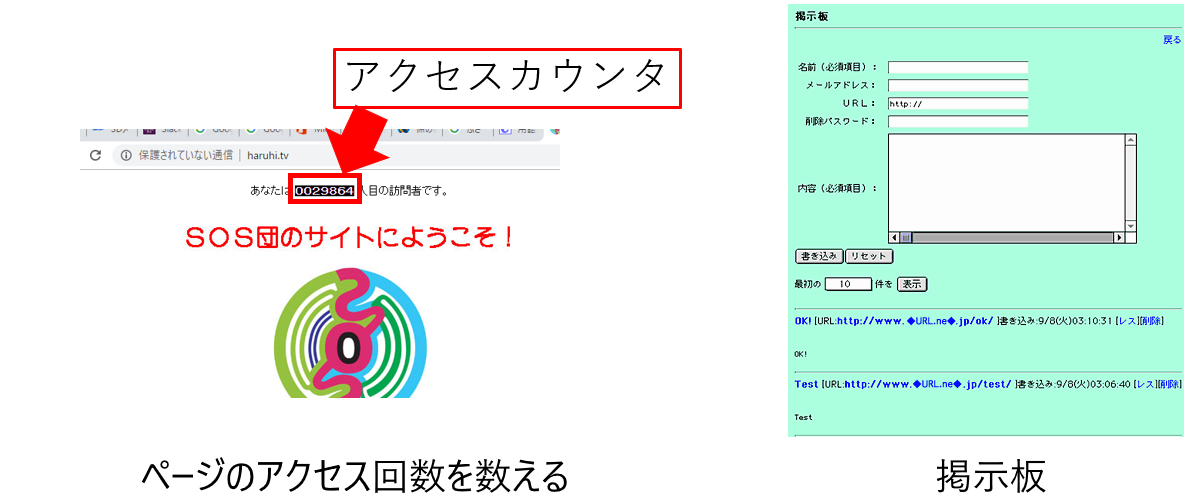
\includegraphics[width=\textwidth]{./slide07-img/slide07-img008.png}}
        \end{minipage}
\end{frame}

\begin{frame}[fragile]
	\frametitle{CGIをりかいしよう\\テキスト P.\pageref{1:P:slide_p28}~~~\raisebox{-3mm}{
\includegraphics[width=0.06\textwidth]{./slide07-img/raspberry.png}}}
        \begin{itemize}\small
            \item 第1回でつくった自己紹介ページのような、HTMLのみのWebページは毎回同じものが帰ってきます。
            \item HTML+CGIの場合、クライアントからの要求のたびにCGIプログラムがHTMLを作成するため、毎回違うWebページが返ってきます。
        \end{itemize}
        \begin{minipage}{\textwidth}
            {\upshape
              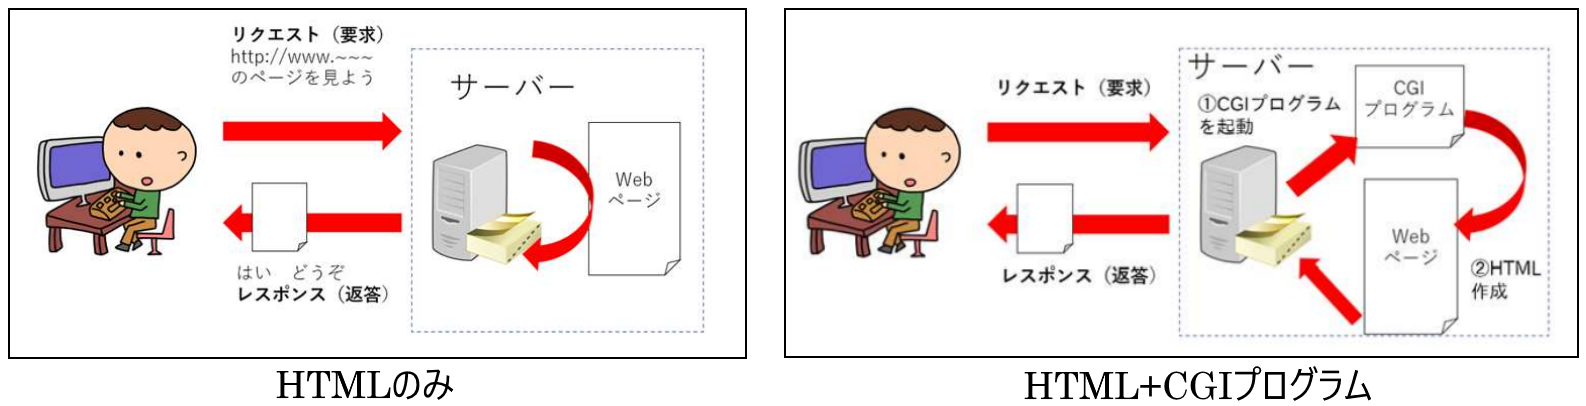
\includegraphics[width=\textwidth]{./slide07-img/slide07-img010.png}}
        \end{minipage}
\end{frame}

\begin{frame}[fragile]
	\frametitle{CGIをつかってみよう\\テキスト P.\pageref{1:P:slide_p28}~~~\raisebox{-3mm}{
\includegraphics[width=0.06\textwidth]{./slide07-img/raspberry.png}}}
      \large\textbf{教科書をよみながら、問題をやってみよう}
				\begin{itemize}\small
					\item \ref*{1:Q:dynamicPage} P.\pageref{1:Q:dynamicPage}
					\item \ref*{1:E:CGI} P.\pageref{1:E:CGI}
					\item \ref*{1:E:URL} P.\pageref{1:E:URL}
					\item \ref*{1:E:QS}  P.\pageref{1:E:QS}
				\end{itemize}
      \vfill
      \large\textbf{わからないことは、放っておかず、すぐに TA に聞きましょう}
\end{frame}
